% ---------- Training with FP8 ----------
\section{Training with \texorpdfstring{FP8}{FP8}}

\subsection{Hardware}
All experiments were executed on a single \textbf{NVIDIA H100 NVL} equipped with 94 GB of HBM3. Its fourth-generation Tensor Cores expose native FP8 arithmetic, which we access through the NVIDIA Transformer Engine (TE) library\cite{transformer_engine}.

\subsection{Training Configuration}
\vspace{-0.5em}
\begin{table}[htbp]
    \centering\small
    \begin{tabular}{lcc}
        \toprule
        \textbf{Hyper-parameter} & \textbf{FP8/BF16 run} & \textbf{FP32 baseline}\\
        \midrule
        Training examples                & 260 K & 260 K\\
        Epochs                           & 3     & 3\\
        Batch size per device            & 26    & 12\\
        Maximum sequence length          & 512   & 512\\
        Gradient-accumulation steps      & 4     & 4\\
        \bottomrule
    \end{tabular}
    \caption{Key hyper-parameters for training the 1.5 B-parameter model.}
    \label{tab:fp8_config}
\end{table}

\subsection{Converting the Pre-trained Model to Transformer Engine Layers}
The publicly available \texttt{qwen2.5} checkpoint from Hugging Face is rewritten by substituting every \texttt{nn.Linear}, \texttt{LayerNorm}, and \texttt{RMSNorm} module with its TE analog. Figure~\ref{fig:te_conversion} sketches this one-to-one mapping, which preserves the original parameter tensors while enabling FP8 kernels.

\begin{figure}[h]
    \centering
    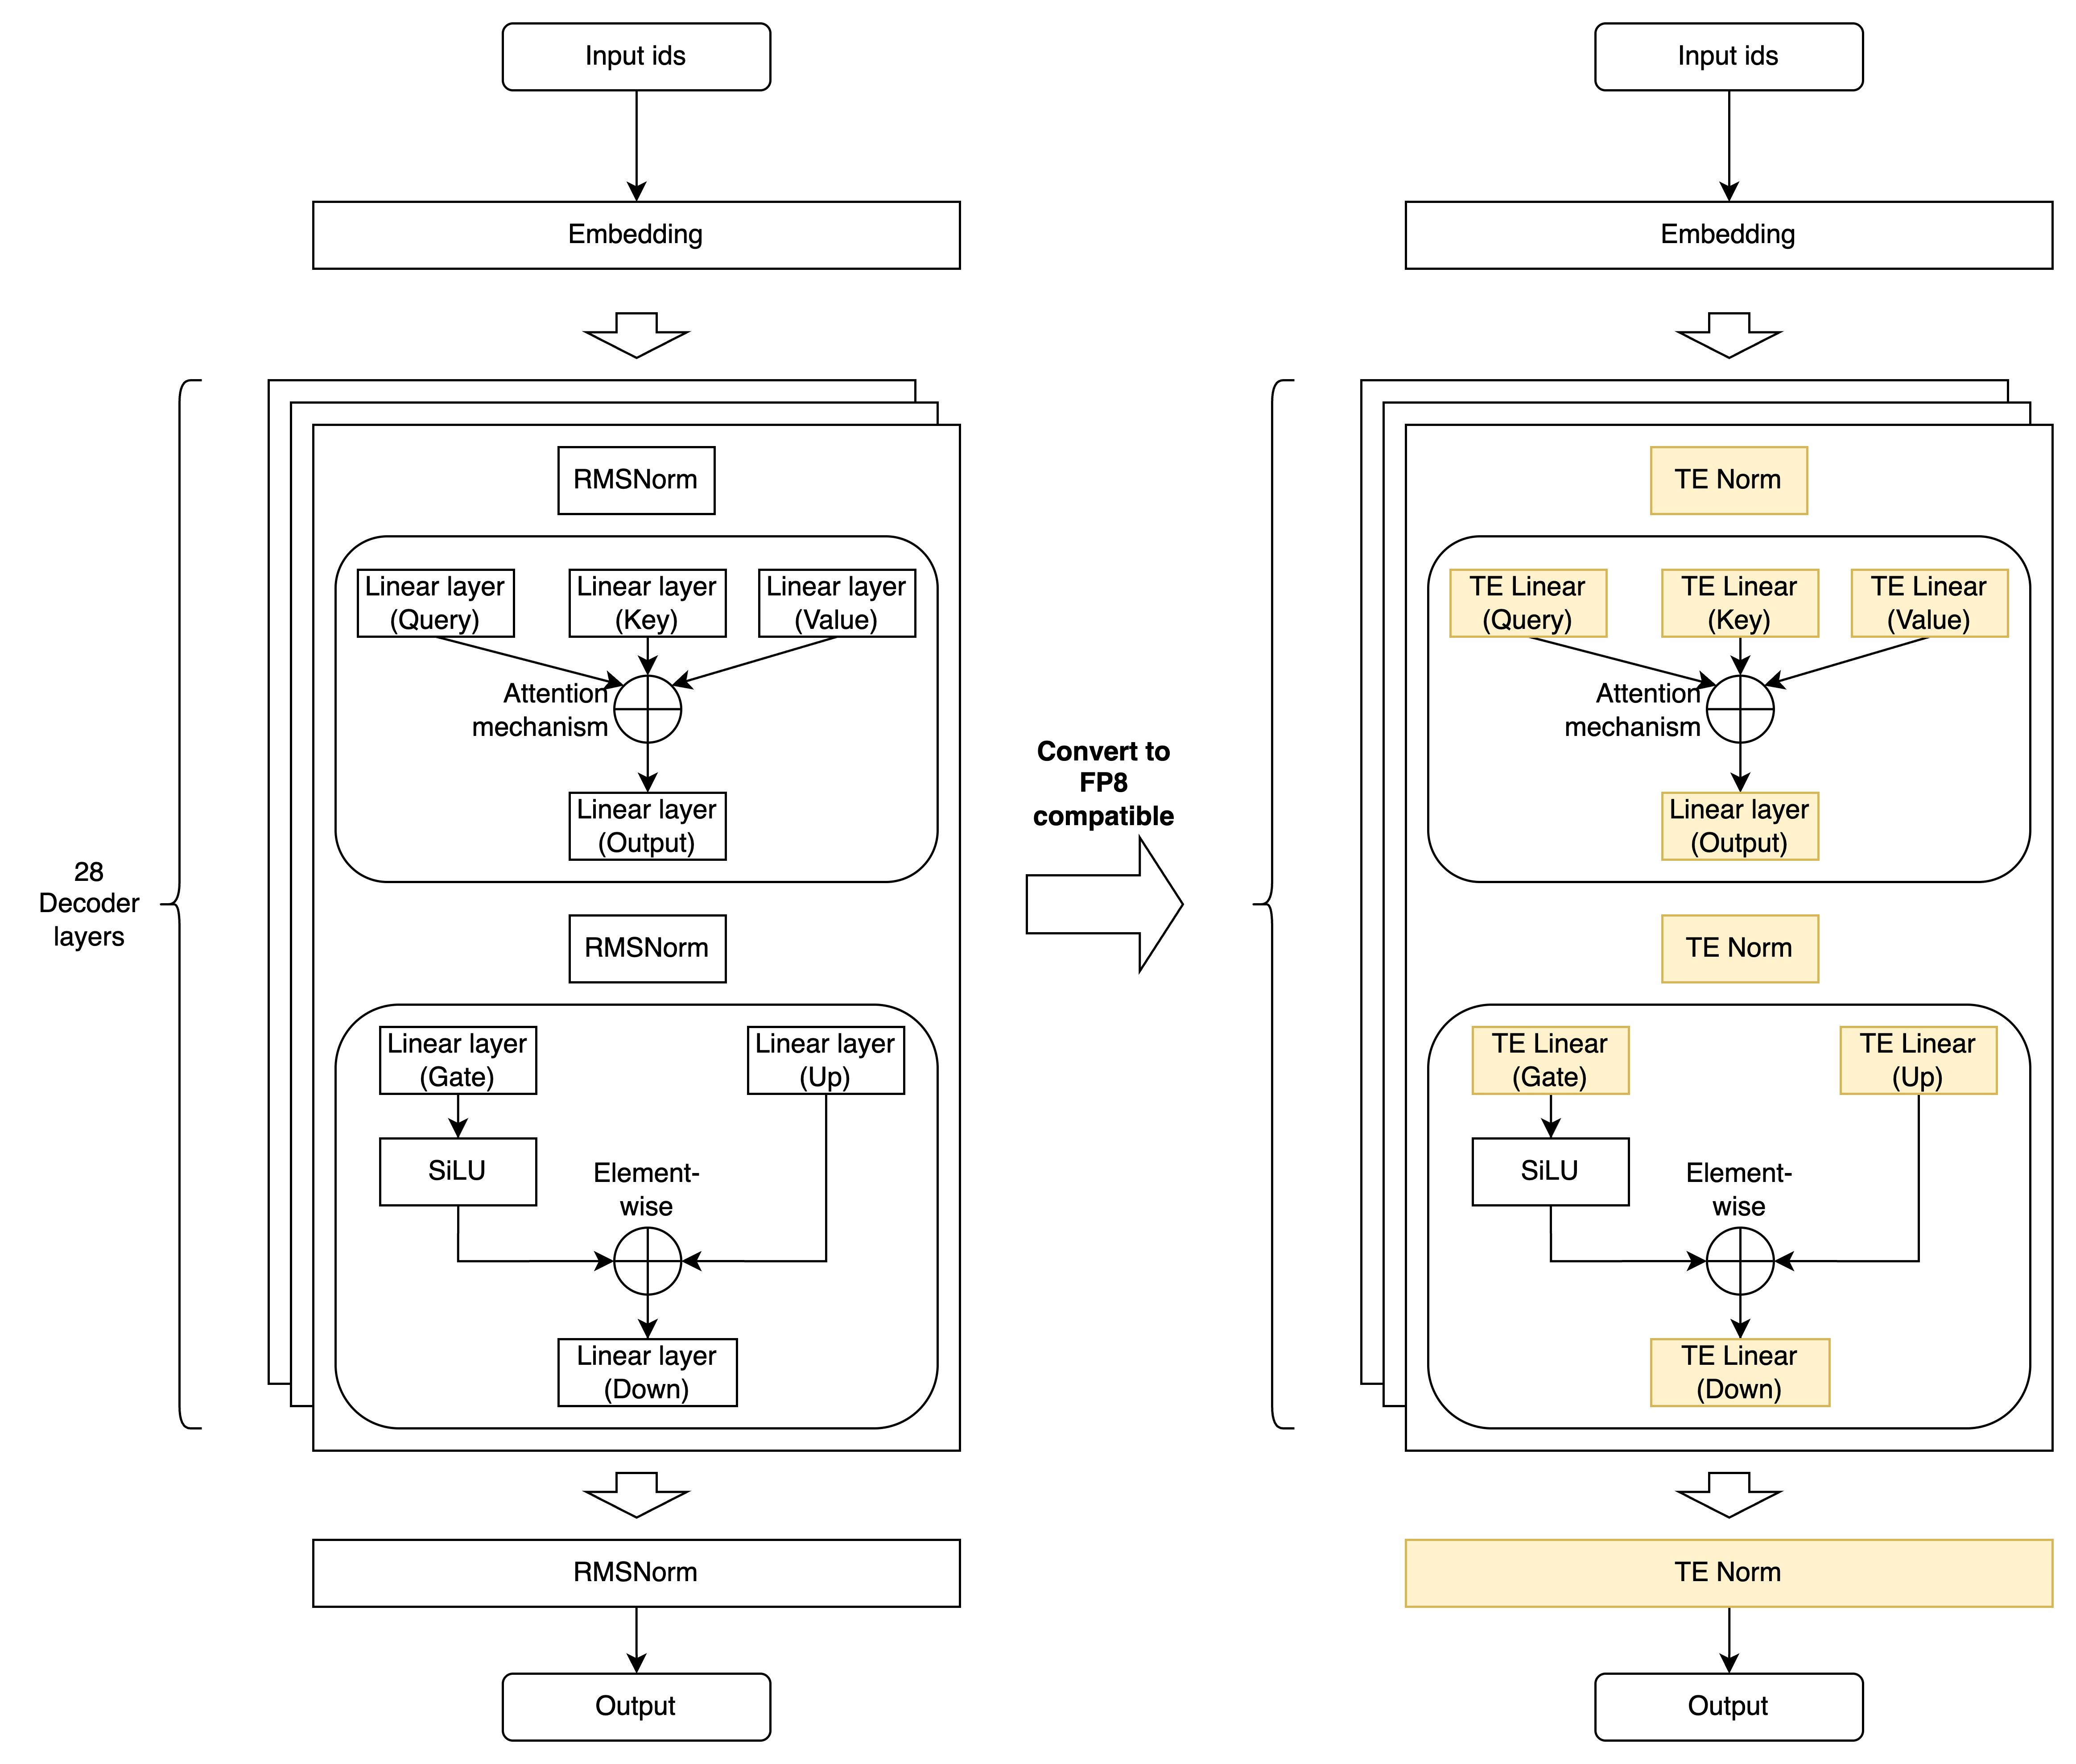
\includegraphics[width=\linewidth]{figures/c3/conversation.drawio.png}
    \caption{Mapping PyTorch layers to NVIDIA Transformer Engine layers.}
    \label{fig:te_conversion}
\end{figure}

\subsection{Precision Recipes}\label{sec:precision_recipes}
We train the model with 3 types of recipes:
\textbf{Hybrid (E4M3/E5M2).}
Weights and forward activations are stored in the \textbf{E4M3} format, whereas gradient buffers use \textbf{E5M2}. The optimizer retains a full-precision (FP32) copy of the weights.

\textbf{Pure E4M3.}
Both weights and forward activations and all gradient buffers reside in \textbf{E4M3}. The optimizer again maintains FP32 master weights to guarantee numerical stability.

\textbf{BF16 Baseline.}
For comparison, we train a BF16 model in which weights, activations, and gradients remain in \textbf{BF16}; only the optimizer state is kept in FP32.

\subsection{Dynamic Scaling Mechanism}
To maintain numerical stability during FP8 training, we implement a dynamic scaling mechanism that adapts to the numerical range of tensors. This is critical because the limited range of FP8 would otherwise lead to frequent overflow or underflow.

\begin{equation}
    \text{FP8}_{\text{tensor}} = \text{round}(\text{tensor} \times \text{scale\_factor})
\end{equation}

The scale factors are computed using a combination of techniques:

\begin{itemize}
    \item \textbf{History-based scaling}: Scale factors are derived from an exponential moving average of recent tensor statistics, with varying window sizes (128 for forward passes, 64 for backward gradients).
    \item \textbf{Margin-based amax calculation}: Maximum absolute values (\textit{amax}) are multiplied by a margin factor (1.1 for weights, 1.3 for activations) to provide headroom for outliers.
    \item \textbf{Format-specific scaling}: Different scaling strategies are applied to E4M3 and E5M2 formats based on their representable ranges.
\end{itemize}

\subsection{Implementation of FP8 Matrix Multiplications}

For each matrix multiplication operation, we implement the following sequence:

\begin{enumerate}
    \item \textbf{Precompute scale factors}: Before training begins, we perform a calibration pass on a small batch of data to initialize scale factors.
    \item \textbf{Cast to FP8}: During each forward pass, tensors are converted to FP8 using the current scale factors:
    \begin{verbatim}
    fp8_weight = cast_to_fp8(weight * weight_scale)
    fp8_input = cast_to_fp8(input * input_scale)
    \end{verbatim}
    
    \item \textbf{Perform FP8 matrix multiplication}: The multiplication is executed using Tensor Cores' FP8 capability:
    \begin{verbatim}
    fp8_output = matmul(fp8_input, fp8_weight)
    \end{verbatim}
    
    \item \textbf{Dequantize the result}: The result is scaled back to higher precision:
    \begin{verbatim}
    output = fp8_output / (input_scale * weight_scale)
    \end{verbatim}
    
    \item \textbf{Update scale factors}: After each iteration, scale factors are updated based on observed tensor statistics.
\end{enumerate}

\subsection{Numerical Stability Considerations}\label{sec:numerical_stability}

Several techniques were employed to maintain numerical stability with FP8:

\begin{itemize}
    \item \textbf{Layer-specific scaling}: Different scale factors are computed for each layer to accommodate varying numerical distributions.
    \item \textbf{Operation selectivity}: Only matrix multiplications use FP8, while other operations such as activations, additions, and normalizations remain in higher precision (BF16).
    \item \textbf{Delayed scaling updates}: Scale factors are updated every 16 iterations to prevent oscillations.
    \item \textbf{Gradient clipping}: We apply a global norm gradient clipping of 1.0 to prevent extreme gradient values.
    \item \textbf{FP32 master weights}: The optimizer maintains a full-precision copy of weights to accumulate small gradient updates that would be lost in lower precision.
\end{itemize}

\subsection{Transformer Engine Configuration}

We configure the Transformer Engine with the following settings to optimize for the Qwen2.5 architecture:

\begin{verbatim}
transformer_engine.common.recipe.DelayedScaling(
    fp8_format=transformer_engine.common.recipe.Format.HYBRID,
    amax_history_len=128,
    amax_compute_algo="max",
    scaling_factor_compute_algo="combined",
    scaling_factor_rounding="nearest",
    fp8_margin=0.95,
    amax_forward_update_margin=1.3,
    amax_backward_update_margin=1.1,
    scaling_factor_update_margin=0.9,
)
\end{verbatim}

This configuration balances numerical stability with computational efficiency, allowing the model to maintain accuracy while benefiting from FP8's performance advantages.

% ---------- End of section ----------
